% replace all text with your own text.
% in this template few examples are mention
\chapter{Methodology}
\label{ch:method} % Label for method chapter

We mentioned in Chapter~\ref{ch:anal_teo} %[example backward reference to a chapter or section.]
that a project report's structure could follow a particular paradigm. Hence, the organization of a report (effectively the Table of Content of a report) can vary depending on the type of project you are doing. Check which of the given examples suit your project. Alternatively, follow your supervisor's advice.

\section{Examples of the sections of a methodology chapter}
A general report structure is summarised (suggested) in Table~\ref{tab:gen_template}. Table~\ref{tab:gen_template} describes that, in general, a typical report structure has three main parts: (1) front matter, (2) main text, and (3) end matter. %[\textbf{also notice that the preceding sentence is an example of a numbered list in a text body}]. 
The structure of the front matter and end matter will remain the same for all the undergraduate final year project report. However, the main text varies as per the project's needs.
\begin{table}[!ht]
    \centering
    \caption{Undergraduate report template structure}
    \label{tab:gen_template}
    \begin{tabular}{llll}     
        \toprule
        \multirow{7}{3cm}{Frontmatter} 
        & & Title Page & \\                  
        & & Abstract &    \\          
        & & Acknowledgements & \\                            
        & & Table of Contents &    \\                                
        & & List of Figures   &    \\                        
        & & List of Tables    &    \\                
        & & List of Abbreviations  &    \\                     
        & &   &    \\                        
        \multirow{7}{3cm}{Main text}
        & Chapter 1 & Introduction   &    \\                         
        & Chapter 2 & Literature Review   &    \\
        & Chapter 3 & Methodology   &    \\
        & Chapter 4 & Results    &    \\
        & Chapter 5 & Discussion and Analysis  &    \\
        & Chapter 6 & Conclusions and Future Work  &    \\        
        & Chapter 7 & Refection  &    \\          
        & &   &    \\                       
        \multirow{2}{3cm}{End matter}
        & & References  &    \\   
        & & Appendices (Optional)  &    \\ 
        & & Index (Optional)  &    \\ 
        \bottomrule
    \end{tabular}
\end{table}

\subsection{Example of a software/Web development main text structure}
\label{subsec:se_chpters}
Notice that the ``methodology'' Chapter of Software/Web development in Table~\ref{tab:soft_eng_temp} takes a standard software engineering paradigm (approach). Alternatively, these suggested sections can be the chapters of their own. Also, notice that ``Chapter 5'' in Table~\ref{tab:soft_eng_temp} is ``Testing and Validation'' which is different from the general report template mentioned in Table~\ref{tab:gen_template}. Check with your supervisor if in doubt.
\begin{table}[!ht]
    \centering
    \caption{Example of a software engineering-type report structure}
    \label{tab:soft_eng_temp}
    \begin{tabular}{lll}     
        \toprule                   
        Chapter 1 & Introduction   &    \\        
        Chapter 2 & Literature Review  &    \\                   
        Chapter 3 & Methodology   &    \\
        &               & Requirements specifications   \\
        &               & Analysis   \\
        &               & Design   \\
        &               & Implementations   \\
        Chapter 4 & Testing and Validation  &    \\
        Chapter 5 & Results and Discussion      &    \\
        Chapter 6 & Conclusions and Future Work  &    \\        
        Chapter 7 & Reflection  &    \\                          
        \bottomrule
    \end{tabular}
\end{table}

\subsection{Example of an algorithm analysis main text structure}
Some project might involve the implementation of a state-of-the-art algorithm and its performance analysis and comparison with other algorithms. In that case, the suggestion in Table~\ref{tab:algo_temp} may suit you the best. 
\begin{table}[!ht]
    \centering
    \caption{Example of an algorithm analysis type report structure}
    \label{tab:algo_temp}
    \begin{tabular}{lll}     
        \toprule                   
        Chapter 1 & Introduction  &    \\        
        Chapter 2 & Literature Review  &    \\                
        Chapter 3 & Methodology   &    \\
        &               & Algorithms descriptions  \\
        &               & Implementations   \\
        &               & Experiments design   \\
        Chapter 4 & Results       &  \\
        Chapter 5 & Discussion and Analysis  &    \\
        Chapter 6 & Conclusion and Future Work  &    \\        
        Chapter 7 & Reflection  &    \\          
        \bottomrule
    \end{tabular}
\end{table}

\subsection{Example of an application type main text structure}
If you are applying some algorithms/tools/technologies on some problems/datasets/etc., you may use the methodology section prescribed in Table~\ref{tab:app_temp}.  
\begin{table}[!ht]
    \centering
    \caption{Example of an application type report structure}
    \label{tab:app_temp}
    \begin{tabular}{lll}     
        \toprule                   
        Chapter 1 & Introduction  &    \\        
        Chapter 2 & Literature Review  &    \\                
        Chapter 3 & Methodology   &    \\
        &               & Problems (tasks) descriptions  \\
        &               & Algorithms/tools/technologies/etc. descriptions  \\        
        &               & Implementations   \\
        &               & Experiments design and setup   \\
        Chapter 4 & Results       &  \\
        Chapter 5 & Discussion and Analysis  &    \\
        Chapter 6 & Conclusion and Future Work  &    \\        
        Chapter 7 & Reflection  &    \\          
        \bottomrule
    \end{tabular}
\end{table}

\subsection{Example of a science lab-type main text structure}
If you are doing a science lab experiment type of project, you may use the  methodology section suggested in Table~\ref{tab:lab_temp}. In this kind of project, you may refer to the ``Methodology'' section as ``Materials and Methods.''
\begin{table}[!ht]
    \centering
    \caption{Example of a science lab experiment-type report structure}
    \label{tab:lab_temp}
    \begin{tabular}{lll}     
        \toprule                   
        Chapter 1 & Introduction  &    \\        
        Chapter 2 & Literature Review  &    \\                
        Chapter 3 & Materials and Methods   &    \\
        &               & Problems (tasks) description  \\
        &               & Materials \\        
        &               & Procedures  \\                
        &               & Implementations   \\
        &               & Experiment set-up   \\
        Chapter 4 & Results       &  \\
        Chapter 5 & Discussion and Analysis  &    \\
        Chapter 6 & Conclusion and Future Work  &    \\        
        Chapter 7 & Reflection  &    \\          
        \bottomrule
    \end{tabular}
\end{table}

\section{Example of an Equation in \LaTeX}
Eq.~\ref{eq:eq_example} [note that this is an example of an equation's in-text citation] is an example of an equation in \LaTeX. In Eq.~\eqref{eq:eq_example}, $ s $ is the mean of elements $ x_i \in \mathbf{x} $: 

\begin{equation}
\label{eq:eq_example} % label used to refer the eq in text
s = \frac{1}{N} \sum_{i = 1}^{N} x_i. 
\end{equation}

Have you noticed that all the variables of the equation are defined using the \textbf{in-text} maths command \$.\$, and Eq.~\eqref{eq:eq_example} is treated as a part of the sentence with proper punctuation? Always treat an equation or expression as a part of the sentence. 

\section{Example of a Figure in \LaTeX}
Figure~\ref{fig:chart_a} is an example of a figure in \LaTeX. For more details, check the link:

\href{https://en.wikibooks.org/wiki/LaTeX/Floats,_Figures_and_Captions}{wikibooks.org/wiki/LaTeX/Floats,\_Figures\_and\_Captions}.

\noindent
Keep your artwork (graphics, figures, illustrations) clean and readable. At least 300dpi is a good resolution of a PNG format artwork. However, an SVG format artwork saved as a PDF will produce the best quality graphics. There are numerous tools out there that can produce vector graphics and let you save that as an SVG file and/or as a PDF file. One example of such a tool is the ``Flow algorithm software''. Here is the link for that: \href{http://www.flowgorithm.org/download/}{flowgorithm.org}.
\begin{figure}[!ht]
    \centering
    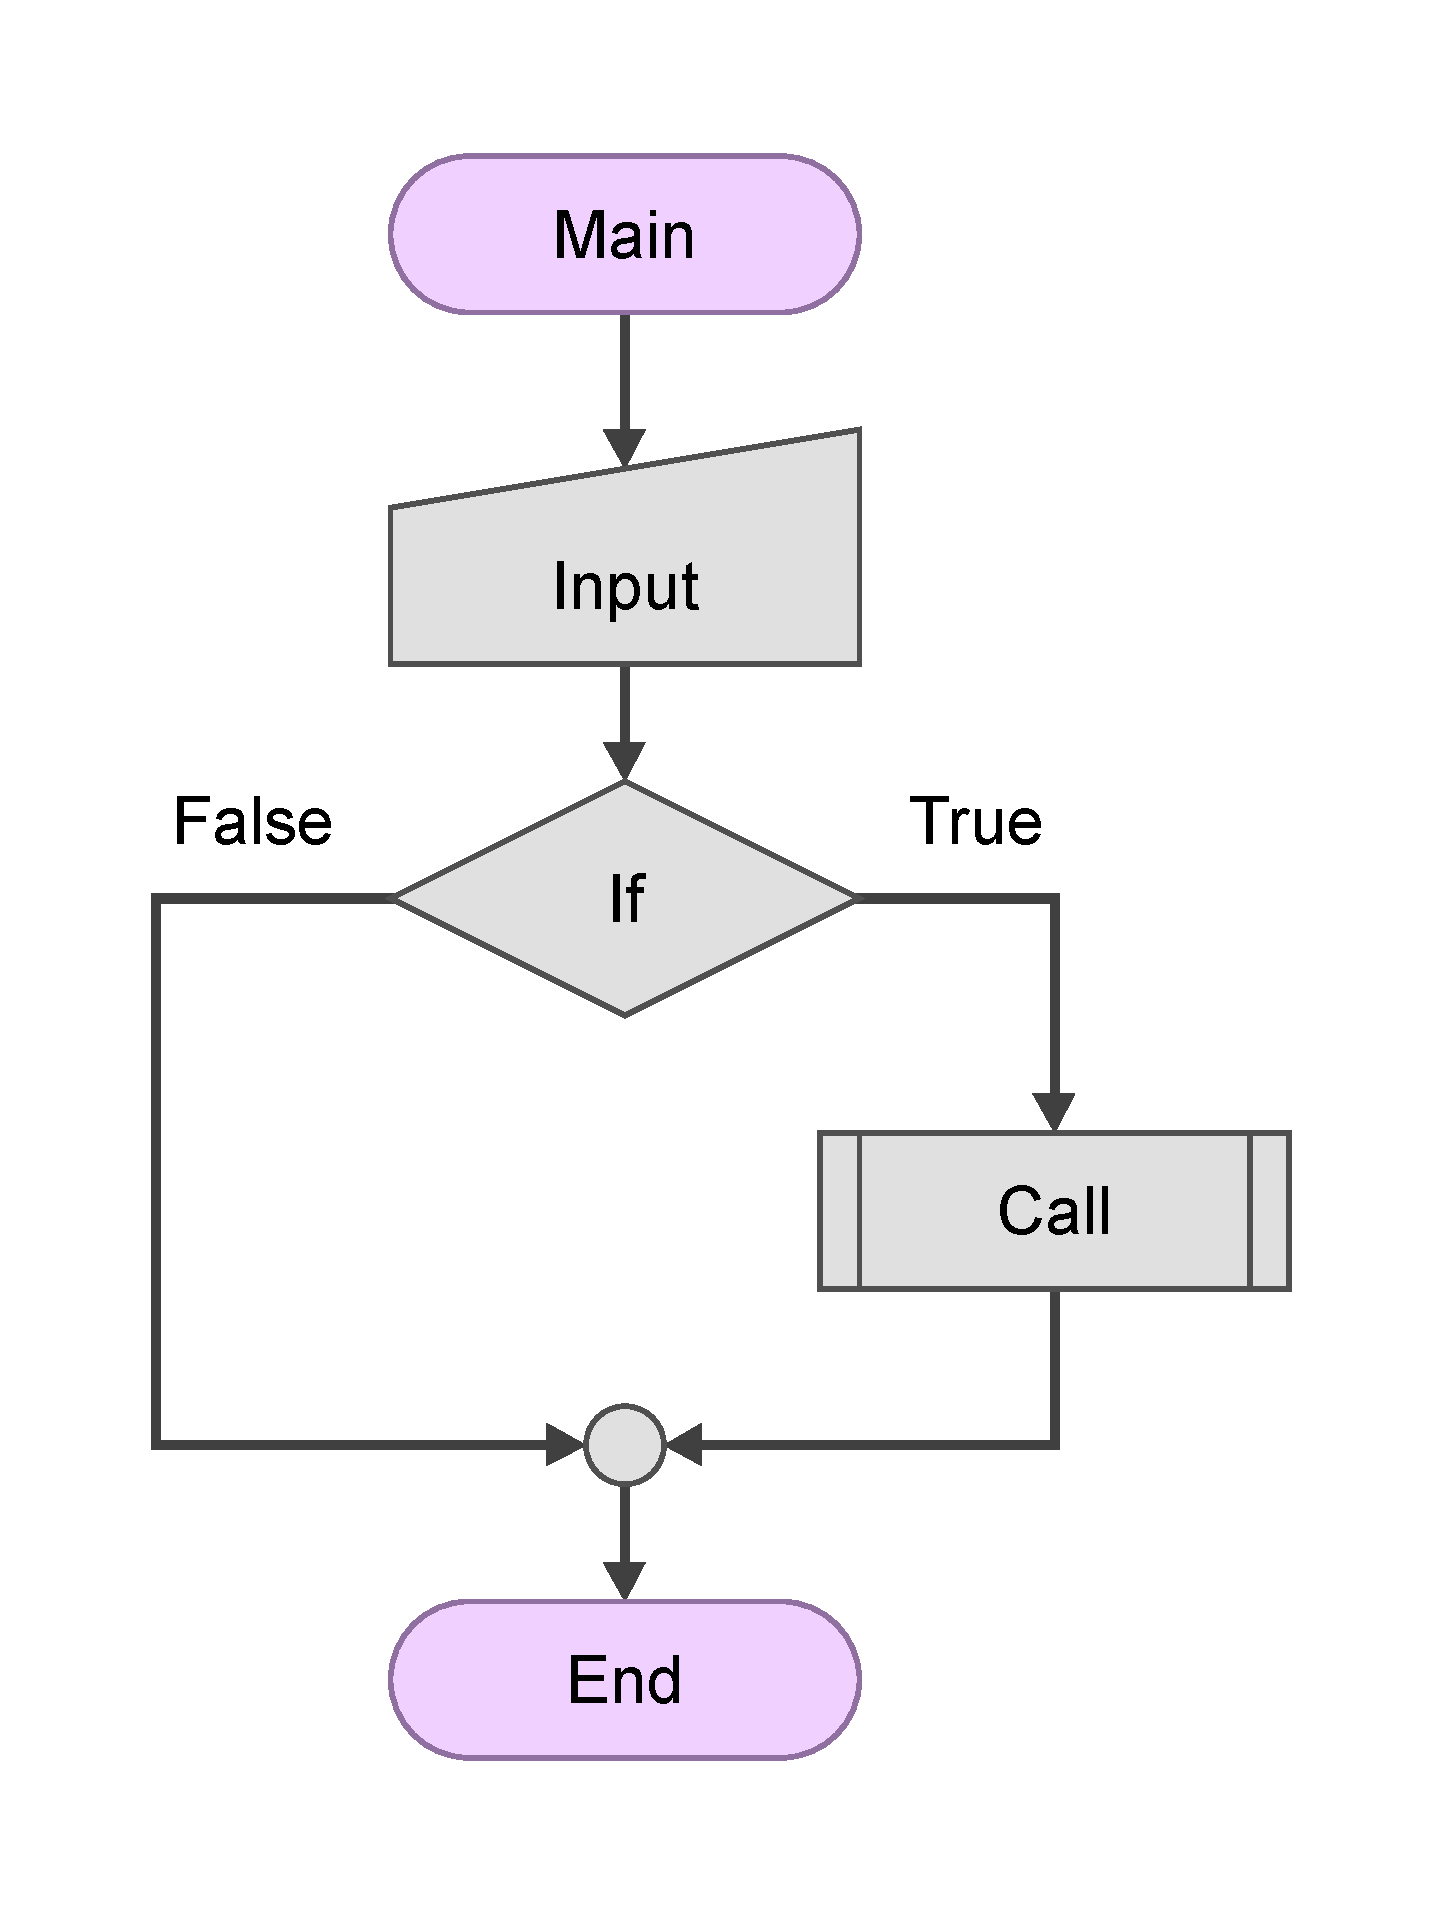
\includegraphics[scale=0.3]{figures/chart.pdf}
    \caption{Example figure in \LaTeX.}
    \label{fig:chart_a}
\end{figure}

\clearpage %  use command \clearpage when you want section or text to appear in the next page.

\section{Example of an algorithm in \LaTeX}
Algorithm~\ref{algo:algo_example} is a good example of an algorithm in \LaTeX.  
\begin{algorithm}
    \caption{Example caption: sum of all even numbers}
    \label{algo:algo_example}
    \begin{algorithmic}[1]
        \Require{$ \mathbf{x}  = x_1, x_2, \ldots, x_N$}
        \Ensure{$EvenSum$ (Sum of even numbers in $ \mathbf{x} $)}
        \Statex
        \Function{EvenSummation}{$\mathbf{x}$}
        \State {$EvenSum$ $\gets$ {$0$}}
        \State {$N$ $\gets$ {$length(\mathbf{x})$}}
        \For{$i \gets 1$ to $N$}                    
        \If{$ x_i\mod 2 == 0$}  \Comment Check whether a number is even.
        \State {$EvenSum$ $\gets$ {$EvenSum + x_i$}}
        \EndIf
        \EndFor
        \State \Return {$EvenSum$}
        \EndFunction
    \end{algorithmic}
\end{algorithm}
 
\section{Example of code snippet  in \LaTeX}

Code Listing~\ref{list:python_code_ex} is a good example of including a code snippet in a report. While using code snippets, take care of the following:
\begin{itemize}
    \item do not paste your entire code (implementation) or everything you have coded. Add code snippets only. 
    \item The algorithm shown in Algorithm~\ref{algo:algo_example} is usually preferred over code snippets in a technical/scientific report. 
    \item Make sure the entire code snippet or algorithm stays on a single page and does not overflow to another page(s).  
\end{itemize}

Here are three examples of code snippets for three different languages (Python, Java, and CPP) illustrated in Listings~\ref{list:python_code_ex}, \ref{list:java_code_ex}, and \ref{list:cpp_code_ex} respectively.  

\begin{lstlisting}[language=Python, caption={Code snippet in \LaTeX ~and  this is a Python code example}, label=list:python_code_ex]
import numpy as np

x  = [0, 1, 2, 3, 4, 5] # assign values to an array
evenSum = evenSummation(x) # call a function

def evenSummation(x):
    evenSum = 0
    n = len(x)
    for i in range(n):
        if np.mod(x[i],2) == 0: # check if a number is even?
            evenSum = evenSum + x[i]
    return evenSum
\end{lstlisting}

Here we used  the ``\textbackslash clearpage'' command and forced-out the second listing example onto the next page. 
\clearpage  %
\begin{lstlisting}[language=Java, caption={Code snippet in \LaTeX ~and  this is a Java code example}, label=list:java_code_ex]
public class EvenSum{ 
    public static int evenSummation(int[] x){
        int evenSum = 0;
        int n = x.length;
        for(int i = 0; i < n; i++){
            if(x[i]%2 == 0){ // check if a number is even?
                evenSum = evenSum + x[i];
            }
        }
        return evenSum;     
    }
    public static void main(String[] args){ 
        int[] x  = {0, 1, 2, 3, 4, 5}; // assign values to an array
        int evenSum = evenSummation(x);
        System.out.println(evenSum);
    } 
} 
\end{lstlisting}


\begin{lstlisting}[language=C, caption={Code snippet in \LaTeX ~and  this is a C/C++ code example}, label=list:cpp_code_ex]
int evenSummation(int x[]){
    int evenSum = 0;
    int n = sizeof(x);
    for(int i = 0; i < n; i++){
        if(x[i]%2 == 0){ // check if a number is even?
            evenSum = evenSum + x[i];
    	}
    }
    return evenSum;     
}

int main(){
    int x[]  = {0, 1, 2, 3, 4, 5}; // assign values to an array
    int evenSum = evenSummation(x);
    cout<<evenSum;
    return 0;
}
\end{lstlisting}



\section{Example of in-text citation style}
\subsection{Example of the equations and illustrations placement and reference in the text}
Make sure whenever you refer to the equations, tables, figures, algorithms,  and listings for the first time, they also appear (placed) somewhere on the same page or in the following page(s). Always make sure to refer to the equations, tables and figures used in the report. Do not leave them without an \textbf{in-text citation}. You can refer to equations, tables and figures more them once.

\subsection{Example of the equations and illustrations style}
Write \textbf{Eq.} with an uppercase ``Eq`` for an equation before using an equation number with (\textbackslash eqref\{.\}). Use ``Table'' to refer to a table, ``Figure'' to refer to a figure, ``Algorithm'' to refer to an algorithm and ``Listing'' to refer to listings (code snippets). Note that, we do not use the articles ``a,'' ``an,'' and ``the'' before the words Eq., Figure, Table, and Listing, but you may use an article for referring the words figure, table, etc. in general.

For example, the sentence ``A report structure is shown in \textbf{the} Table~\ref{tab:gen_template}'' should be written as ``A report structure is shown \textbf{in} Table~\ref{tab:gen_template}.'' 
 

\section{Summary}
Write a summary of this chapter.

~\\[5em]
\noindent
{\huge\textbf{Note:}} In the case of \textbf{software engineering} project a Chapter ``\textbf{Testing and Validation}'' should precede the ``Results'' chapter. See Section~\ref{subsec:se_chpters} for report organization of such project. 

